\chapter{Spanning Trees}
Rishnak found Ajur and Jura walking along a stretch of road with trees on either side. Recalling his previous talks with Ajur about trees, Rishnak chose a specific kind of tree in a graph for his next session with Ajur.
In a connected graph $G=(V,E)$ (connected means that there is a path between every pair of vertices in $G$), a tree (spanning all the vertices) is a sub-graph =$T(V,E_1)$ of G satisfying the two conditions:
\begin{enumerate}
    \item The sub-graph, T,  is a tree. (i.e., contains no cycles and of course connected; i.e., there is only one path between every pair of vertices.)
    \item Vertex set of $T$ is the same as the vertex set of $G$.
\end{enumerate}

Here is an example of graph Figure \ref{11g1} and a sub-graph of this graph, which is a spanning tree shown in Figure \ref{11g2} 
\begin{figure}
\begin{center}
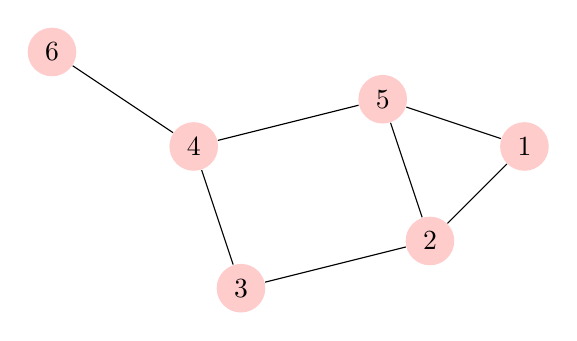
\begin{tikzpicture}
  [scale=.6,auto=left,every node/.style={circle,fill=red!20}]
  \node (n6) at (1,10) {6};
  \node (n4) at (4,8)  {4};
  \node (n5) at (8,9)  {5};
  \node (n1) at (11,8) {1};
  \node (n2) at (9,6)  {2};
  \node (n3) at (5,5)  {3};

  \foreach \from/\to in {n6/n4,n4/n5,n5/n1,n1/n2,n2/n5,n2/n3,n3/n4}
    \draw (\from) -- (\to);

\end{tikzpicture}
\caption{ Example graph with 6 vertices and 7 edges}\label{11g1}
\end{center}
\end{figure}
\begin{figure}
\begin{center}
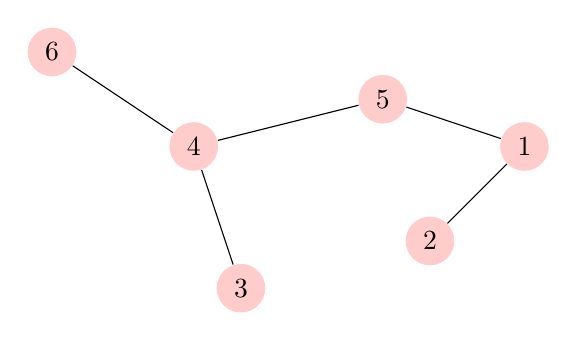
\begin{tikzpicture}
  [scale=.6,auto=left,every node/.style={circle,fill=red!20}]
  \node (n6) at (1,10) {6};
  \node (n4) at (4,8)  {4};
  \node (n5) at (8,9)  {5};
  \node (n1) at (11,8) {1};
  \node (n2) at (9,6)  {2};
  \node (n3) at (5,5)  {3};

  \foreach \from/\to in {n6/n4,n4/n5,n5/n1,n1/n2,n3/n4}
    \draw (\from) -- (\to);

\end{tikzpicture}
\caption{ Sub-graph of Figure \ref{11g1}, which is a spanning tree of \ref{11g1} - Spanning tree has 6 vertices and 5 edges}\label{11g2}
\end{center}
\end{figure}
Rishnak asked Ajur if he could construct one more spanning tree for this graph \ref{11g1}. Ajur was eager to show off and drew the following graph \ref{11g3}.
\begin{figure}
\begin{center}
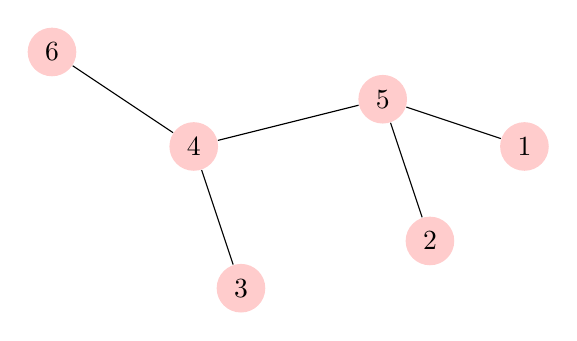
\begin{tikzpicture}
  [scale=.6,auto=left,every node/.style={circle,fill=red!20}]
  \node (n6) at (1,10) {6};
  \node (n4) at (4,8)  {4};
  \node (n5) at (8,9)  {5};
  \node (n1) at (11,8) {1};
  \node (n2) at (9,6)  {2};
  \node (n3) at (5,5)  {3};

  \foreach \from/\to in {n6/n4,n4/n5,n5/n1,n2/n5,n3/n4}
    \draw (\from) -- (\to);

\end{tikzpicture}
\caption{ Another spanning tree of the graph in Figure \ref{11g1}}\label{11g3}
\end{center}
\end{figure}

Rishnak then asked Ajur how many distinct spanning trees (labelled non isomorphic) there are. Ajur had a quick answer this time too. There are two cycles in this graph, namely (2,3,4,5) and (1,5,2). One is of 
length 4 and the other is of length 3. But they share a common edge (2,5). There are 4 possible spanning trees to choose from the cycle of length 4 and there are 3 possibilities to choose from the other cycle - giving rise to 12 possibilities. But one of them contains a cycle \{if (edge (5,2) omitted in the 4 cycle and in the 3 cycle\}; thus giving rise to 11  spanning trees. They are enumerated.   
The edge (4,6) has to be present in every spanning tree. The eleven spanning tree edges are given below.
\begin{enumerate}
    \item \{(4,6),(4,5),(5,2),(2,3),(5,1)\}
    \item \{(4,6),(4,5),(5,2),(2,3),(2,1)\}
    \item \{(4,6),(4,5),(4,3),(5,2),(5,1)\}
    \item \{(4,6),(4,5),(4,3),(5,2),(2,1)\}
    \item \{(4,6),(4,3),(2,3),(5,2),(5,1)\}
    \item \{(4,6),(4,3),(2,3),(5,2),(2,1)\}
    \item \{(4,6),(4,5),(4,3),(2,3),(5,1)\}
    \item \{(4,6),(4,5),(4,3),(2,3),(2,1)\}
    \item \{(4,6),(4,5),(2,3),(5,1),(1,2)\}
    \item \{(4,6),(4,5),(4,3),(5,1),(1,2)\}
    \item \{(4,6),(4,3),(3,2),(2,1),(1,5)\}
\end{enumerate}

Ajur asked what the maximum number of labeled spanning trees is is n a graph with $n$ vertices. Ajur added that the maximum number of spanning trees will be present in a complete graph as it has the maximum number of edges in a $n$ vertex graph. Rishnak agreed that complete graphs have the largest number of spanning trees. We can find the number of spanning trees in a complete graph using Pr{\"u}fer code (which we talked about a couple of days ago) in Chapter 8. Ajur remembered it and interjected for a $n$ vertex tree, one needed only a Pr{\"u}fer code of length $n-2$. Rishnak agreed and said that the Pr{\"u}fer code is of length $n-2$ for a $n$ vertex graph. Each of the $n-2$ characters in a code to be any of the $n$ vertices. Hence the number of (labeled) spanning trees in a complete graph with $n$ vertices is $n^{n-2}$.

Since there are $n-1$ edges in a spanning tree, each of the remaining $e-n+1$ edges when taken with a spanning tree will create a cycle. Thus there will be $e-n+1$ cycles. These cycles are called Fundamental cycles. Each fundamental cycle has exactly one 
non-spanning tree edge.\footnote{Euler's equation \ref{eqn:euler} in chapter 9 uses this fact.} Rishnak showed with an example Figure \ref{11g4}.

\begin{figure}
\begin{center}
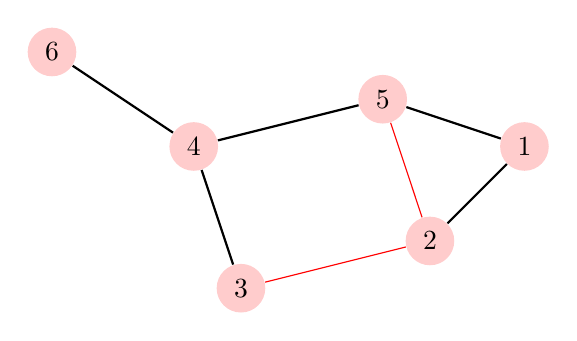
\begin{tikzpicture}
  [scale=.6,auto=left,every node/.style={circle,fill=red!20}]
  \node (n6) at (1,10) {6};
  \node (n4) at (4,8)  {4};
  \node (n5) at (8,9)  {5};
  \node (n1) at (11,8) {1};
  \node (n2) at (9,6)  {2};
  \node (n3) at (5,5)  {3};

  \foreach \from/\to in {n6/n4,n4/n5,n5/n1,n1/n2,n3/n4}
    \draw [thick] (\from) -- (\to);
  \foreach \from/\to in {n5/n2,n2/n3}
   \draw [color=red] (\from) -- (\to);
\end{tikzpicture}
\caption{ Two fundamental cycles of \ref{11g1} with respect to a spanning tree of \ref{11g2} - Spanning tree edges are shown as thick lines and non-spanning tree edges are shown in red color. Fundamental Cycles are (1,2,5) and (4,5,1,2,3)}\label{11g4}
\end{center}
\end{figure}

Ajur wanted to know from Rishnak how to find a spanning tree for a given graph. Rishnak said that the graph has to be connected.\footnote{Between every pair of vertices there is a path.} It can be done using the following steps.
\begin{figure} 
\begin{enumerate}
\item Start from any vertex. Include that vertex in a bag.
\item From the vertices in a bag, find a vertex, $v$, (not in a bag) that is adjacent to one of the vertices, $w$, in the bag. Include that edge, $(v,w)$ in the spanning tree.
\item Repeat the above step till all the vertices are in the bag.
\end{enumerate}
\caption{Finding a Spanning Tree Procedure}\label{11a1}
\end{figure}
Rishnak illustrated his procedure for the example in Figure \ref{11g1}.
Put vertex labeled 1 in the bag. Its adjacent vertices are labeled 2 and 5. Choose vertex (the choice is arbitrary) labeled 5 and put in the bag. Edge (1,5) is included in the spanning tree. From vertices in the bag find a vertex that is adjacent (but not in the bag). Choices are either vertices labeled 2 or 4. Choose the vertex labeled 2 and include edge (1,2) in the spanning tree. (We could have also included (5,2) instead of (1,2) in the spanning tree.). Now the bag contains the vertices (1, 2, 5). Find a vertex that is adjacent to any of these vertices (that are not in the bag). They are namely vertices labeled 4 and 3. Choose (this choice is arbitrary) the vertex labeled 4 and include the edge (4,5) in the spanning tree. Now vertices (1,2,4,5) are in the bag. From these vertices find a vertex that is adjacent but not in the bag. They will be 6 and 3.  Choose the vertex labeled 3 and include the edge (4,3) in the spanning tree. The bag contains the vertices (1,2,3,4,5). The vertex that is adjacent to one
of the vertices in the bag is labeled 6. Choose that vertex labeled 6 and include the edge (4,6) in the spanning tree. Now the bag contains all the vertices and we have the spanning tree edges (1,5), (1,2), (5,4), (4,3) and (4,6). This is the same spanning tree shown in Figure \ref{11g2}.

If we had made different choices, we will get a different spanning tree as shown in Figure \ref{11g3}.

A graph is weighted if there are weights associated with an edge. The weight could represent the distance in miles or the cost of travel etc. Here is an example of a weighted graph with the weighted edges.
\begin{figure}
\begin{center}
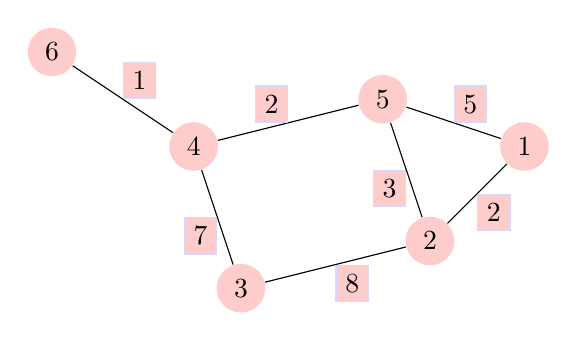
\begin{tikzpicture}
  [scale=.6,auto=left,every node/.style={circle,fill=red!20}]
  \tikzstyle{weight} = [draw=blue!15,shape=rectangle]
  \node (n6) at (1,10) {6};
  \node (n4) at (4,8)  {4};
  \node (n5) at (8,9)  {5};
  \node (n1) at (11,8) {1};
  \node (n2) at (9,6)  {2};
  \node (n3) at (5,5)  {3};
  \foreach \source /\dest /\weight in {n6/n4/1,n4/n5/2,n5/n1/5,n1/n2/2,n2/n5/3,n2/n3/8,n3/n4/7} 
   \draw (\source) --node[weight] {$\weight$}  (\dest);
\foreach \source /\dest /\weight in {1/3/1} place \weight above of=\path;
  
  \end{tikzpicture}
\caption{ Example of a weighted graph with 6 vertices and 7 edges - weights are associated with edges}\label{11g7}
\end{center}
\end{figure}

Rishnak then told Ajur of an interesting problems - to find a minimum spanning tree in a weighted graph. In other words find a spanning tree where the sum of all the edge weights (in a spanning tree) is the smallest. Ajur responded saying one can enumerate all spanning trees and compute for each spanning tree the sum of weights and choose the spanning tree with the smallest sum of edge weights. Rishnak smiled on hearing about the  "Brute Force" method - a good strategy that can work for most problems. The problem is to find out if there are more efficient methods.\footnote{Informally a faster method that makes choices so that one does not have to consider at all spanning trees.} We can adapt/modify the procedure/method described in Figure \ref{11a1} as follows.
\begin{figure} 
\begin{enumerate}
\item Start from any vertex. Include that vertex in a bag.
\item From the vertices in a bag, find a vertex, $v$, (not in a bag) that is adjacent to one of the vertices, $w$, in the bag and with the smallest edge weight $(v,w)$. Include that edge in the minimum spanning tree.
\item Repeat the above step till all the vertices are in the bag.
\end{enumerate}
\caption{Finding a  minimum spanning tree procedure}\label{11aa}
\end{figure}

Ajur chose to work through the example shown in Figure \ref{11g7}. He choose vertex labeled 1 in the bag. Then the vertex labeled 2 is put in the bag as the edge weight (1,2) is the smallest from vertex labeled 1. Now vertices labeled 1 and 2 are in the bag. Edge (2,5) is the smallest edge weight and hence (2,5) is included in the minimum spanning tree and vertex labeled 5 is put in the bag. Among vertices in the bag, namely 1, 2 and 5, the edge (5,4) has the smallest weight. Now the bag contains vertices labeled 1,2,5 and 4. The edge (4,6) is the smallest weight. Hence vertex labeled 6 is included in the bag and edge (4,6) is added to the minimum spanning tree. Edge (4,7) is the smallest weight and hence edge (4,7) is  included in the minimum spanning tree. Now the bag contains all the vertices and hence Ajur exclaimed that he found the minimum spanning tree.
Ajur drew the minimum spanning tree in the following Figure \ref{11g8}

\begin{figure}
\begin{center}
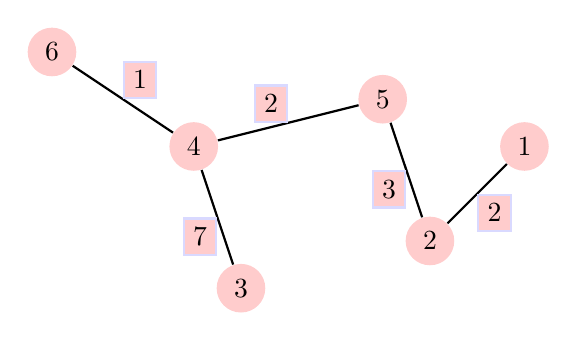
\begin{tikzpicture}
  [scale=.6,auto=left,every node/.style={circle,fill=red!20}]
  \tikzstyle{weight} = [draw=blue!15,shape=rectangle]
  \node (n6) at (1,10) {6};
  \node (n4) at (4,8)  {4};
  \node (n5) at (8,9)  {5};
  \node (n1) at (11,8) {1};
  \node (n2) at (9,6)  {2};
  \node (n3) at (5,5)  {3};
  \foreach \source /\dest /\weight in {n6/n4/1,n4/n5/2,n1/n2/2,n2/n5/3,n3/n4/7} 
   \draw[thick] (\source) --node[weight] {$\weight$}  (\dest);
\foreach \source /\dest /\weight in {1/3/1} place \weight above of=\path;
  
  \end{tikzpicture}
\caption{ Minimum spanning tree of the weighted Graph\ref{11g7}}\label{11g8}
\end{center}
\end{figure}

Ajur could not control his enthusiasm and exclaimed that he could use this procedure to minimally connect a given set of points in a plane. The distance between these points could be the length of straight lines joining them. Ajur showed his work Figure \ref{11g9}.

\begin{figure}
\begin{center}
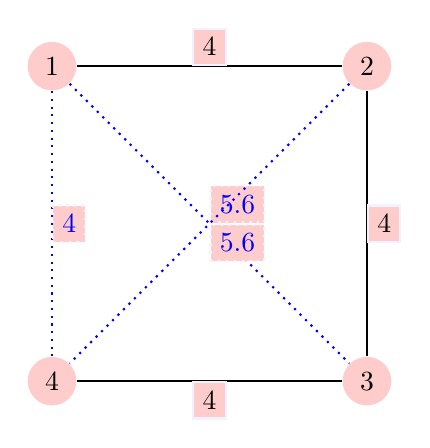
\begin{tikzpicture}
  [scale=1,auto=left,every node/.style={circle,fill=red!20}]
  \tikzstyle{weight} = [draw=blue!5,shape=rectangle]
  \node (n1) at (1,9)  {1};
  \node (n2) at (5,9) {2};
  \node (n3) at (5,5)  {3};
  \node (n4) at (1,5)  {4};
  \foreach \source /\dest /\weight in {n1/n2/4,n2/n3/4,n3/n4/4} 
   \draw[thick] (\source) --node[weight] {$\weight$}  (\dest);
\foreach \source /\dest /\weight in {1/3/1} place \weight above of=\path;
  \foreach \source /\dest /\weight in {n1/n4/4,n1/n3/5.6,n2/n4/5.6} 
   \draw[color=blue,thick,dotted] (\source) --node[weight] {$\weight$}  (\dest);
\foreach \source /\dest /\weight in {1/3/1} place \weight below of=\path;
  \end{tikzpicture}
\caption{ Minimum spanning tree of a set of four points- Non minimum spanning tree edges are drawn as dotted lines}\label{11g9}
\end{center}
\end{figure}

Urpur, another ghost had been eavesdropping on all these conversations. Urpur wanted to show of that he is smarter than both Rishnak and Ajur, so started talking about the spanning tree called Steiner Tree, wherein one is allowed to add Steiner points/vertices that were not present in the original given set of vertices. With a clever addition of Steiner points, one can get a spanning tree, which is smaller than the one Ajur found in \ref{11g9}. Urpur then showed the following Figure \ref{11g10}

\begin{figure}
\begin{center}
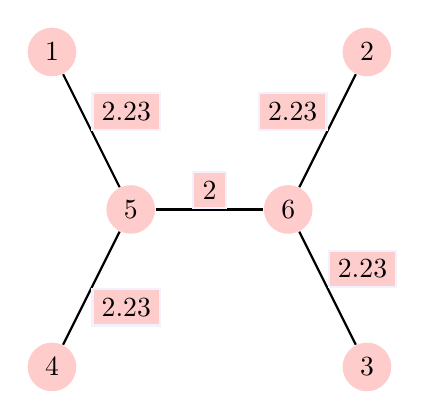
\begin{tikzpicture}
  [scale=1,auto=left,every node/.style={circle,fill=red!20}]
  \tikzstyle{weight} = [draw=blue!5,shape=rectangle]
  \node (n1) at (1,9)  {1};
  \node (n2) at (5,9) {2};
  \node (n3) at (5,5)  {3};
  \node (n4) at (1,5)  {4};
  \node (n5) at (2,7) {5};
  \node (n6) at (4,7) {6};
  \foreach \source /\dest /\weight in {n1/n5/2.23,n5/n6/2,n6/n2/2.23,n6/n3/2.23,n5/n4/2.23} 
   \draw[thick] (\source) --node[weight] {$\weight$}  (\dest);
\foreach \source /\dest /\weight in {1/3/1} place \weight below of=\path;
 
  \end{tikzpicture}
\caption{ Minimum Steiner Tree of a set of four points. Steiner points/vertices are 5 and 6}\label{11g10}
\end{center}
\end{figure}

Rishnak was very impressed with Urpur's thinking. Sensing that Ajur was feeling jealous that Urpur was grabbing his attention,

\textbf{Question for the ninth day}
Rishnak was very impressed with Urpur's thinking. Sensing that Ajur was feeling jealous that Urpur was grabbing his attention, Consider a complete graph with with 8 vertices and 28 edges. 14 of the edges have weight
1 and 14 of the edges have weight 10. Which of the edges have what weights to answer the
following  two questions: 
\begin{enumerate}
    \item Show how to assign weights to the edges so as to achieve the smallest possible weight minimum-weight-spanning tree. What is the smallest weight?
\item Show how to assign weights to the edges so as to achieve the \textbf{largest} possible weight \textbf{minimum weight} spanning tree. What is the largest weight of the minimum-weight-spanning tree.
 
\end{enumerate}

\textbf{Answer:} Ajur could do the first part easily if there is a cycle of length 8, with edge weight being 1, the minimum spanning tree weight will be 7.

Ajur found the second problem a bit more challenging. To get the maximum weight, all edges incident on a vertex have to be of weight 10. That is possible with only two vertices. Hence the maximum weight the minimum spanning tree can have will be 25.


 Rishnak called it a night. Jura was happy now to get Ajur's attention and jumping with joy, left with Ajur.